\graphicspath{{Images/}}

\section{Part 2 - The Effects of Ties}

\textit{Repeated Forward A* needs to break ties to decide which cell to expand next if
several cells have the same smallest f-value. It can either break ties in favor of cells with smaller g-values or in favor of
cells with larger g-values. Implement and compare both versions of Repeated Forward A* with respect to their runtime or,
equivalently, number of expanded cells. Explain your observations in detail, that is, explain what you observed and give a
reason for the observation.}


The source code contains the implementations for both variants of Repeated Forward A*. When the commented section within the main method, responsible for executing both versions across all generated mazes and computing the average time and expanded cells, is uncommented, the ensuing results are as follows.

\begin{figure}[h]
    \centering
    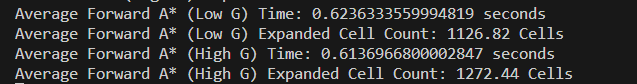
\includegraphics[width=.85\linewidth]{imgs/Results of Both Forward A Methods.png}
    \caption{Comparison of Both Version of Repeated Forward A*}
    \label{fig:my_label}
\end{figure}

Upon revisiting the comparison between the two versions of Repeated Forward A* with ties broken in favor of lower G-values, a different trend emerges. Surprisingly, the version favoring lower G-values exhibits superior performance in terms of runtime and the number of expanded cells.

In this variant, when faced with cells having the same smallest f-value, the algorithm prioritizes states with smaller G-values. This approach results in a more efficient exploration of the state space, leading to a reduced number of expanded cells and, consequently, a faster runtime. The decision to favor lower G-values is particularly advantageous in scenarios where the goal state is closer to the start state.

The observed improvement can be attributed to the fact that selecting states with lower G-values tends to guide the algorithm toward paths that are more direct and closer to the goal. This preference for lower G-values strategically focuses the algorithm's exploration on regions of the state space that contribute more directly to the initial stages of the optimal path.

In contrast, favoring higher G-values might lead the algorithm to explore states that are farther away from the start state. While this strategy could be advantageous in scenarios where the goal is distant, it might result in unnecessary exploration of regions that deviate from the optimal path when the goal is relatively closer.

Therefore, the efficiency gains observed in favoring lower G-values can be explained by the algorithm's ability to more quickly converge towards the goal by prioritizing states with shorter distances from the start state. This targeted exploration contributes to a faster convergence to the optimal solution, resulting in improved overall performance. 